\documentclass{amsart}
\usepackage[utf8]{inputenc}
\usepackage[
backend=biber,
style=alphabetic,
sorting=ynt
]{biblatex}

\addbibresource{TheBib.bib} %Imports bibliography file
\usepackage{tikz}
\usetikzlibrary{arrows}

\newtheorem{thm}{Theorem}[section]
\newtheorem{lemma}[thm]{Lemma}
\newtheorem{prop}[thm]{Proposition}
\newtheorem{corollary}[thm]{Corollary}

\newenvironment{defn}[1][Definition]{\begin{trivlist}
\item[\hskip \labelsep {\bfseries #1}]}{\end{trivlist}}

\newcommand{\R}{\mathbb{R}}
\newcommand{\Y}{\Gamma_Y}
\newcommand{\n}{$n$}

\title{Chapter 3}
\author{Tynan Daly}


\begin{document}
\maketitle
\section{Defining Configuration Space}\label{sec:productspace}

We again turn our attention to the example of the CW complex we just introduced. This ``Y-graph", which we denote as $\Y$, is the simplest non-trivial example of restricted network of robot movement. Other simple graphs have trivial solutions.

\begin{figure}[h]\label{fig:trivial}
\centering
\caption{Examples of Graphs with Trivial Solutions}
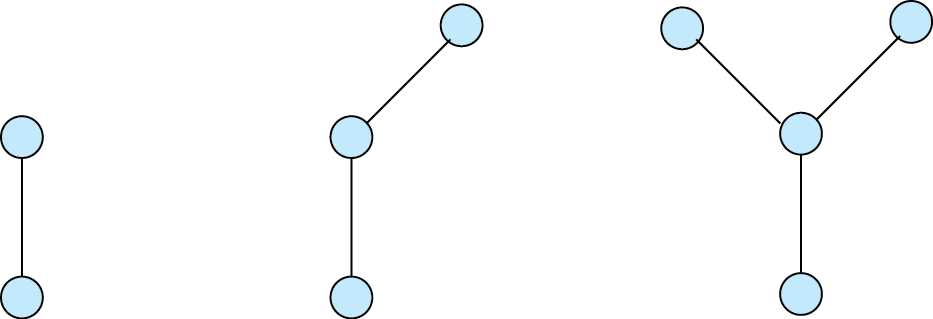
\includegraphics[scale=.5]{Building_Y.png}
\end{figure}


Consider the graph of two vertices connected by an edge as illustrated in Figure~\ref{fig:trivial}. If we have only two robots on this graph, then each of them cannot reach the opposite vertex without collision. Thus, we will attach an additional edge and vertex. However, we again encounter the same problem, so we attach another vertex and edge. Thus we obtain $\Y$. 

\begin{figure}[h]
\caption{The graph $\Y$}
\centering
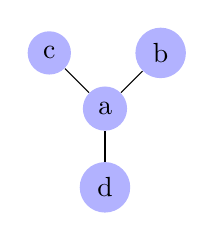
\begin{tikzpicture}
  [scale=.7,auto=left,every node/.style={circle,fill=blue!30}]
  \node (n1) {a};
  \node (n2) [above right of=n1]  {b};
  \node (n3) [above left of=n1] {c};
  \node (n4) [below of=n1] {d};

\foreach \from/\to in
{n1/n3,n2/n1,n4/n1}
    \draw (\from) -> (\to);
\end{tikzpicture}
\label{fig:maze}
\end{figure}

So that we may have an interesting problem, we choose to work with $\Y$ as labeled in Figure~\ref{fig:maze}. When there is one robot moving about $\Y$ the solution is trivial since there is nothing for the robot to collide with. It is only when we add an additional robot that things become interesting. 

\begin{defn}
Given a space $X$ with $N$ robots, the configuration space, $C^N(X)$ is defined as $C^N(X)= (\underbrace{X \times X\times \dots \times X}_{N \text{ times} }) - \Delta$ where $$\Delta = \{(x_1, x_2, \dots, x_N) \in X | x_i =x_j \text{ for some } i \neq j\}.$$ 
\end{defn}

Each point in the configuration space $C^N(X)$ is a distinct configuration of $N$ robots at distinct points in $X$, where the robots are labeled $1$, $2$, $\ldots$, $N$ so that $x_i$ is the position of robot $i$ in the space $X$. 

Let us consider two robots which can only move backwards and forwards in a straight line. For these robots, their movement space is $\R$. Thus their configuration space is $C^2(\R) = [\R\times \R]- \{(x_1,x_2)\in \R | x_1 = x_2\}$. Clearly the first part of the configuration space is the plane $\R^2$ where each point represents our two robots' positions on $\R$. The point $(1,3)$, for instance, would mean that robot one is at position one and robot two is at position three in $\R$. However, to obtain our configuration space, we must remove $\Delta$. What are the points in the movement space which represent a collision? They are the points where $x_1=x_2$, and so for this example, they are all the points on the line $y=x$. Thus, removing $\Delta$ ensures that the points in the configuration space are positions where the two robots cannot collide in $\R$.

\begin{figure}[h]\label{fig:xygraph}
\centering
\caption{$C^2(\R)$}
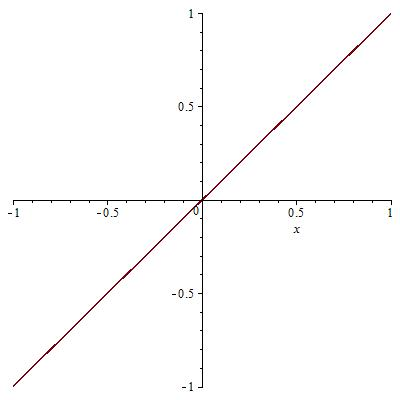
\includegraphics[scale=.25]{Presentation/xygraph.jpg}
\end{figure}



Each time we introduce a new robot to our space we must take another product of their movement space. Adding a new robot to our previous example would yield $C^3(\R)=\R^3 - \{(x_1,x_2,x_3)\in \R^3|x_i=x_j \text{ for some } i \neq j\}$. 

The configuration space $C^2(\R)$, as seen in Figure~
\ref{fig:xygraph} is easy to visualize, but we include it in order to give us a solid foundation when we consider more complicated spaces. Consider, for example,  robots which may move around freely in two-dimensions, such as self-driving cars. The configuration space of two self-driving cars moving around a flat open field would be $C^2(\R^2)= [\R^2 \times \R^2]-\Delta$. As we can see, the problem of collision avoidance quickly escapes our ability to visualize even the simplest non-trivial case and so obscures solutions from our intuition. 

We, however, are not interested with robots moving around a flat plane. Considerable work has been done on this problem. For more information about provably safe configuration spaces we refer readers to Koditschek and Rimon \cite{safe}. Our interest lies in finite networks, such as tracks or guided wires, which robots can move around. As a result, we will examine $\Y$ and its configuration space.

The examples of robots moving about $\R^2$ is hard to visualize, but not necessarily hard to construct. We have been working with $\R^2$ for years and so many of us have a good grasp on the space's properties, but this is not the case for $\Y$. We will construct $C^2(\Y)$ through CW complexes, but we will proceed carefully due to the complexity involved. Recall that the configuration space is defined as $C^2(\Y)~=~(Y\times Y)~-~\Delta$. We begin constructing the configuration space by first building the product space $\Y \times \Y$.

\section{Building the Product Space}

From Chapter 2, we know that graphs are one-dimensional CW complexes composed of $0$ and $1$ cells. The product space of two one-dimensional CW-complexes is a two-dimensional CW-complex, and so to construct the product CW-complex we take the cross product of each cell in the first complex with each cell in the second complex. In the graph $\Y$, we have the $0$-cells $a,b$ and the one cell $(a,b)$. To demonstrate the process for constructing $\Y \times \Y$, let us take the product space of the CW complexes below. Note the subscript on each vertex denotes the position of the first and second robot. 

\begin{figure}[h]
\caption{A sub-graph of $\Y$.}\label{fig:subgraph}
\centering
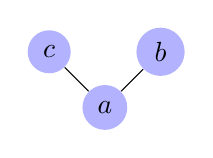
\begin{tikzpicture}
  [scale=.7,auto=left,every node/.style={circle,fill=blue!30}]
  \node (n1) {$a$};
  \node (n2) [above right of=n1]  {$b$};
  \node (n3) [above left of=n1] {$c$};
  \foreach \from/\to in
{n1/n2, n1/n3}
    \draw (\from) -> (\to);
\end{tikzpicture}
\hspace{1in}
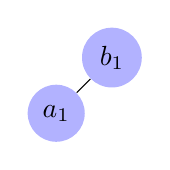
\begin{tikzpicture}
  [scale=.7,auto=left,every node/.style={circle,fill=blue!30}]
  \node (n1) {$a_1$};
  \node (n2) [above right of=n1]  {$b_1$};

\foreach \from/\to in
{n1/n2}
    \draw (\from) -> (\to);
\end{tikzpicture}
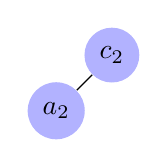
\begin{tikzpicture}
  [scale=.7,auto=left,every node/.style={circle,fill=blue!30}]
  \node (n1) {$a_2$};
  \node (n2) [above right of=n1]  {$c_2$};

\foreach \from/\to in
{n1/n2}
    \draw (\from) -> (\to);
\end{tikzpicture}
\end{figure}

We will begin by considering the subgraph of $\Gamma_{Y}$ represented in the left side of Figure~\ref{fig:subgraph}. Let robot one be interested in only moving between positions $a$ and $b$ and let robot two only be interested in moving between positions $a$ and $c$. We represent this visually by the right-hand side of Figure~\ref{fig:subgraph}. We label each vertex by the robot which could be on it, thus $a_1$ is the point where robot one is at position $a$ and $c_2$ is the point where robot two is at position $c$. We should be careful to note that even though we choose to represent our graph in this way in order to simplify the construction of the product $2$-cell, $a_1$ and $a_2$ both represent the same vertex.

To construct the product space, we will follow a series of steps similar to the construction of CW Complexes in Chapter 2. We begin with the collection of $0$-cells, $X^0$. Since our product space consists of the cross product of $\Y$, our vertices in the product space will be the cross product of the $0$-cells as seen in Figure~\ref{fig:vertexcross}. Each vertex is a configuration of robots on $\Y$. For example, $a_1c_2$ is the point where robot one is at $a$ \textit{and} robot two is at $c$.

\begin{figure}[h]
\caption{Cross Product of Vertices}\label{fig:vertexcross}
\centering
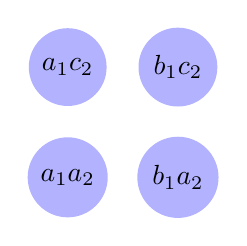
\begin{tikzpicture}
  [scale=.7,auto=left,every node/.style={circle,fill=blue!30}]
  \node (n1) at (1,3)  {$a_1c_2$};
  \node (n2) at (3,3)  {$b_1c_2$};
  \node (n3) at (1,1)  {$a_1a_2$};
  \node (n4) at (3,1)  {$b_1a_2$};


\end{tikzpicture}
\end{figure}

Next we take the cross product of the $0$-cells, $a_1$ and $b_1$, with the $1$-cell $(a_2,c_2)$. This will give us two edges vertically connecting the top and bottom vertices with one another. Doing the opposite operation, taking the cross product of $a_2$ and $c_2$ with $(a_1, b_1)$, will give us the two remaining edges. Together, these edges and vertices form the boundary of the $2$-cell.

\begin{figure}[h]
\caption{Cross Product of Vertices and Edges}\label{fig:crosswithedges}
\centering
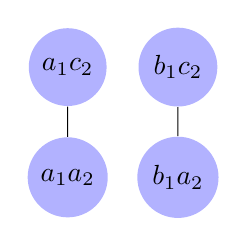
\begin{tikzpicture}
  [scale=.7,auto=left,every node/.style={circle,fill=blue!30}]
  \node (n1) at (1,3)  {$a_1c_2$};
  \node (n2) at (3,3)  {$b_1c_2$};
  \node (n3) at (1,1)  {$a_1a_2$};
  \node (n4) at (3,1)  {$b_1a_2$};
\foreach \from/\to in
{n1/n3, n2/n4}
    \draw (\from) -> (\to);

\end{tikzpicture}
\hspace{.5in}
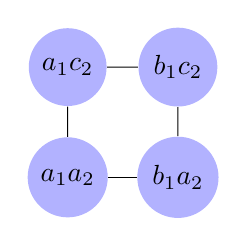
\begin{tikzpicture}
  [scale=.7,auto=left,every node/.style={circle,fill=blue!30}]
  \node (n1) at (1,3)  {$a_1c_2$};
  \node (n2) at (3,3)  {$b_1c_2$};
  \node (n3) at (1,1)  {$a_1a_2$};
  \node (n4) at (3,1)  {$b_1a_2$};

\foreach \from/\to in
{n1/n2, n3/n4, n1/n3, n2/n4}
    \draw (\from) -> (\to);

\end{tikzpicture}
\end{figure}

Intuitively, edges in Figure~\ref{fig:crosswithedges} denote one robot's position between vertices. The edge $(a_1c_2, b_1c_2)$ represents the possible positions of robot one between $a$ and $b$, while robot two remains stationary at $c$.

To finish constructing this product space, we must take the product of both $1$-cells. The space $(a_1,b_1)\times (a_2, c_2)$ is homeomorphic to $B^2$, and so our final space is a closed $2$-cell as seen in Figure~\ref{fig:firsttwocell}. A closed $2$-cell represents all the possible positions of the two robots along two edges. 
 
\begin{figure}[h]
\caption{A Closed $2$-Cell}\label{fig:firsttwocell}
\centering
 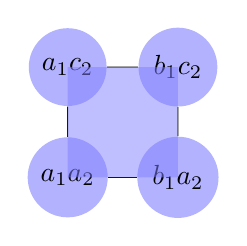
\begin{tikzpicture}
  [scale=.7,auto=left,every node/.style={circle,fill=blue!30}]
  \node (n1) at (1,3)  {$a_1c_2$};
  \node (n2) at (3,3)  {$b_1c_2$};
  \node (n3) at (1,1)  {$a_1a_2$};
  \node (n4) at (3,1)  {$b_1a_2$};

\foreach \from/\to in
{n1/n2, n3/n4, n1/n3, n2/n4}
    \draw (\from) -> (\to);
    \path[fill=blue!50,opacity=.5] (n1.center) to (n2.center) to (n4.center) to (n3.center) to (n1.center);
\end{tikzpicture}
\end{figure}

We can do this again with the $1$-cells $(a_1,d_1)$ and $(a_2, c_2)$ and obtain its product, seen in Figure~\ref{fig:secondcross}, and then we attach it to the $2$-cell in Figure~\ref{fig:firsttwocell} at the corresponding vertices and edges, which gives us the CW-complex in Figure~\ref{fig:firstattaching}. We may then add the $2$-cell formed by $(a_1, d_1) \times (a_2, b_2)$ to form Figure~\ref{fig:thirdattaching}. If we continue this process without crossing any of the $1$-cells with themselves, we will obtain Figure~\ref{fig:base}.

\begin{figure}[h]
\caption{Cross product of  $(a_1, d_1)$ and $(a_2,c_2)$}\label{fig:secondcross}
\centering
 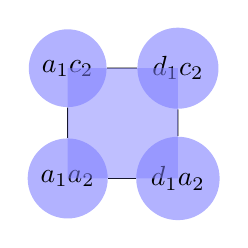
\begin{tikzpicture}
  [scale=.7,auto=left,every node/.style={circle,fill=blue!30}]
  \node (n1) at (1,3)  {$a_1c_2$};
  \node (n2) at (3,3)  {$d_1c_2$};
  \node (n3) at (1,1)  {$a_1a_2$};
  \node (n4) at (3,1)  {$d_1a_2$};

\foreach \from/\to in
{n1/n2, n3/n4, n1/n3, n2/n4}
    \draw (\from) -> (\to);
    \path[fill=blue!50,opacity=.5] (n1.center) to (n2.center) to (n4.center) to (n3.center) to (n1.center);
\end{tikzpicture}
\end{figure}



\begin{figure}[h]
\caption{Attached $2$-Cells}\label{fig:firstattaching}
\centering
 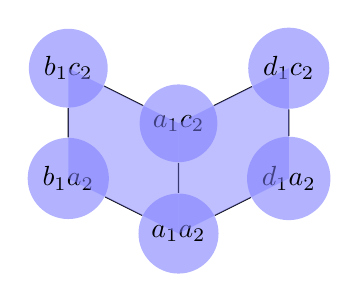
\begin{tikzpicture}
  [scale=.7,auto=left,every node/.style={circle,fill=blue!30}]
  \node (n1) at (1,2)  {$b_1a_2$};
  \node (n2) at (1,4)  {$b_1c_2$};
  \node (n3) at (3,1)  {$a_1a_2$};
  \node (n4) at (3,3)  {$a_1c_2$};
  \node (n5) at (5,4)  {$d_1c_2$};
  \node (n6) at (5,2)  {$d_1a_2$};


\foreach \from/\to in
{n1/n3, n2/n4, n1/n2, n4/n3, n4/n5, n5/n6, n6/n3}
    \draw (\from) -> (\to);
    \path[fill=blue!50,opacity=.5] (n1.center) to (n2.center) to (n4.center) to (n3.center) to (n1.center);
    \path[fill=blue!50,opacity=.5] (n4.center) to (n5.center) to (n6.center) to (n3.center) to (n4.center);
\end{tikzpicture}
\end{figure}



\begin{figure}[h]
\caption{Three Attached $2$-Cells}\label{fig:thirdattaching}
\centering
 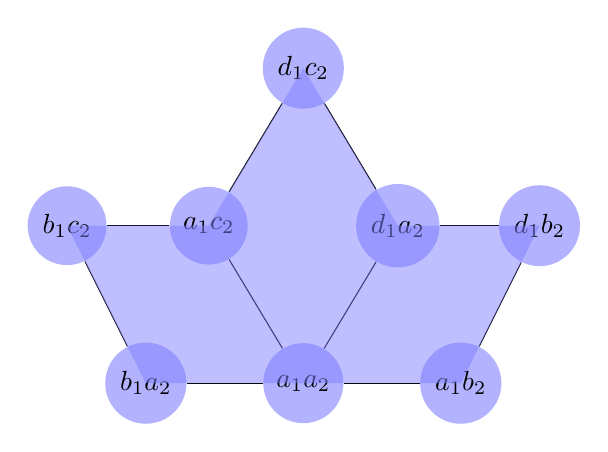
\begin{tikzpicture}
  [scale=1,auto=left,every node/.style={circle,fill=blue!30}]
  \node (n1) at (1,0)    {$b_1a_2$};
  \node (n2) at (0,2)    {$b_1c_2$};
  \node (n3) at (3,0)    {$a_1a_2$};
  \node (n4) at (1.8,2)  {$a_1c_2$};
  \node (n5) at (3,4)    {$d_1c_2$};
  \node (n6) at (4.2,2)  {$d_1a_2$};
  \node (n7) at (6,2)    {$d_1b_2$};
  \node (n8) at (5,0)    {$a_1b_2$};

\foreach \from/\to in
{n1/n3, n2/n4, n1/n2, n4/n3, n4/n5, n5/n6, n6/n3, n6/n7, n7/n8, n8/n3}
    \draw (\from) -> (\to);
    \path[fill=blue!50,opacity=.5] (n1.center) to (n2.center) to (n4.center) to (n3.center) to (n1.center);
    \path[fill=blue!50,opacity=.5] (n4.center) to (n5.center) to (n6.center) to (n3.center) to (n4.center);
    \path[fill=blue!50,opacity=.5] (n3.center) to (n6.center) to (n7.center) to (n8.center) to (n3.center);
\end{tikzpicture}
\end{figure}



\begin{figure}[h]
\caption{Six Attached $2$-Cells}\label{fig:base}
\centering
 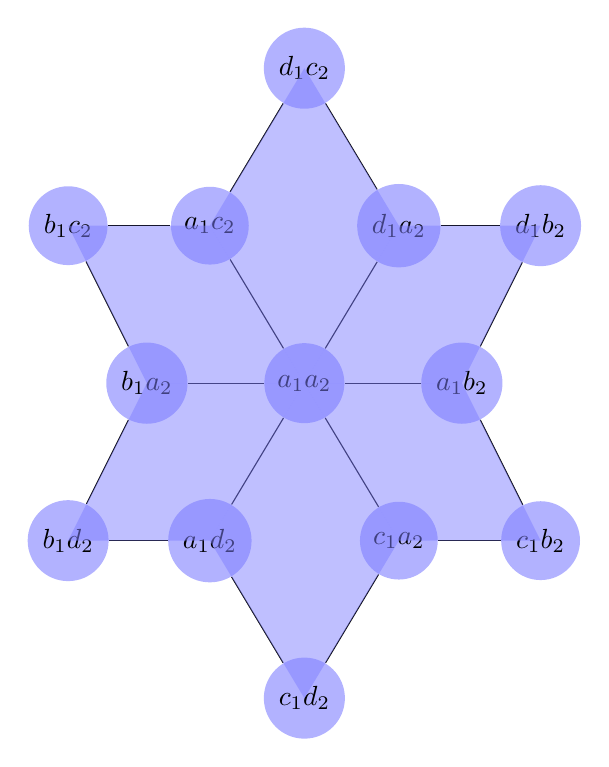
\begin{tikzpicture}
  [scale=1,auto=left,every node/.style={circle,fill=blue!30}]
  \node (n1) at (1,0)       {$b_1a_2$};
  \node (n2) at (0,2)       {$b_1c_2$};
  \node (n3) at (3,0)       {$a_1a_2$};
  \node (n4) at (1.8,2)     {$a_1c_2$};
  \node (n5) at (3,4)       {$d_1c_2$};
  \node (n6) at (4.2,2)     {$d_1a_2$};
  \node (n7) at (6,2)       {$d_1b_2$};
  \node (n8) at (5,0)       {$a_1b_2$};
  
  \node (n9) at (0,-2)      {$b_1d_2$};
  \node (n10) at (1.8, -2)  {$a_1d_2$};
  \node (n11) at (3,-4)     {$c_1d_2$};
  \node (n12) at (4.2, -2)  {$c_1a_2$};
  \node (n13) at (6,-2)     {$c_1b_2$};

\foreach \from/\to in
{n1/n3, n2/n4, n1/n2, n4/n3, n4/n5, n5/n6, n6/n3, n6/n7, n7/n8, n8/n3, n1/n9, n9/n10, n10/n3, n10/n11, n11/n12, n12/n3, n12/n13, n13/n8}
    \draw (\from) -> (\to);
    \path[fill=blue!50,opacity=.5] (n1.center) to (n2.center) to (n4.center) to (n3.center) to (n1.center);
    \path[fill=blue!50,opacity=.5] (n4.center) to (n5.center) to (n6.center) to (n3.center) to (n4.center);
    \path[fill=blue!50,opacity=.5] (n3.center) to (n6.center) to (n7.center) to (n8.center) to (n3.center);
    \path[fill=blue!50,opacity=.5] (n1.center) to (n9.center) to (n10.center) to (n3.center) to (n1.center);
    \path[fill=blue!50,opacity=.5] (n3.center) to (n10.center) to (n11.center) to (n12.center) to (n3.center);
    \path[fill=blue!50,opacity=.5] (n3.center) to (n12.center) to (n13.center) to (n8.center) to (n3.center);
\end{tikzpicture}
\end{figure}

But we are not yet finished. We must now cross all the $1$-cells with themselves. This is where our space becomes messy. In order to visualize this, we will embed the product space in $\R^3$. Figure \ref{fig:productspace} represents all possible moves two robots may make, regardless of whether or not a collision will occur. Since there are three $1$-cells and four $0$-cells in $\Y$, our final product space will consist of $9$ $2$-cells, twenty-four $1$-cells, and sixteen $0$-cells.

\begin{figure}[h]
\caption{$\Y \times \Y$}\label{fig:productspace}
\centering
 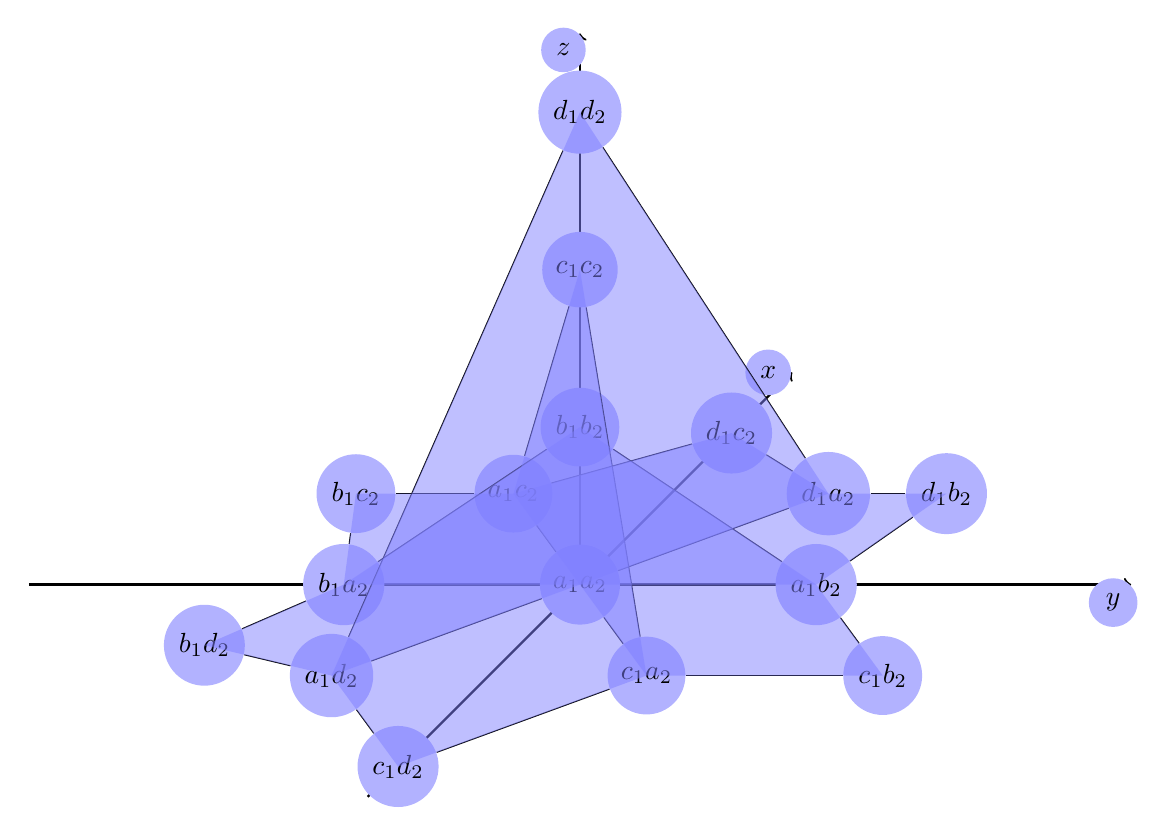
\begin{tikzpicture}
  [scale=1,auto=left,every node/.style={circle,fill=blue!30}]
  \draw[thick,->,black] (-7,0,0) -- (7,0,0) node[anchor=north east]{$y$};
  \draw[thick,->] (0,0,0) -- (0,7,0) node[anchor=north east]{$z$};
  \draw[thick,->] (0,0,7) -- (0,0,-7) node[anchor=east]{$x$};
  
  \node (n0) at (0,0,0)         {$a_1a_2$};
  \node (n1) at (0,0,-5)        {$d_1c_2$};
  \node (n2) at (0,0,6)         {$c_1d_2$};
  \node (n3) at (-3,0,0)        {$b_1a_2$};
  \node (n4) at (3,0,0)         {$a_1b_2$};
  \node (n5) at (-4,0, 2)       {$b_1d_2$};
  \node (n6) at (-2,0, 3)       {$a_1d_2$};
  \node (n7) at (-4,0,-3)       {$b_1c_2$};
  \node (n8) at (-2,0,-3)       {$a_1c_2$};
  \node (n9) at (2,0, 3)        {$c_1a_2$};
  \node (n10) at (5, 0, 3)      {$c_1b_2$};
  \node (n11) at (3.5, 0, -3)   {$d_1b_2$};
  \node (n12) at (2, 0, -3)     {$d_1a_2$};
  \node (n13) at (0, 6, 0)      {$d_1d_2$};
  \node (n14) at (0, 4, 0)      {$c_1c_2$};
  \node (n15) at (0,2,0)        {$b_1b_2$};
  
  \foreach \from/\to in
{n0/n8, n0/n9, n0/n6, n0/n12, n0/n3, n0/n4, n4/n11, n11/n12, n4/n10, n10/n9, n12/n1, n1/n8, n8/n7, n7/n3, n3/n5, n5/n6, n6/n2, n2/n9, n6/n13, n13/n12, n8/n14, n14/n9, n3/n15, n15/n4}
    \draw (\from) -> (\to);
    \path[fill=blue!50,opacity=.5] (n1.center) to (n12.center) to (n11.center) to (n4.center) to (n10.center) to (n9.center) to (n2.center) to (n6.center) to (n5.center) to (n3.center) to (n7.center) to (n8.center) to (n1.center);
    \path[fill=blue!50,opacity=.5] (n6.center) to (n13.center) to (n12.center) to (n6.center);
    \path[fill=blue!50,opacity=.5] (n8.center) to (n14.center) to (n9.center) to (n8.center);
    \path[fill=blue!50,opacity=.5] (n3.center) to (n15.center) to (n4.center) to (n3.center);
\end{tikzpicture}
\end{figure}
\clearpage

\newpage

\newpage
\section{The Configuration Space}

Now that we have the product space of $\Y \times \Y$, we must remove the pairwise diagonal $\Delta$ to complete the construction of the configuration space $C^2(\Y)$. Recall that $\Delta = \{(x_1,x_2,\dots, x_n)\in X | x_i = x_j\text{ for some } i \neq j\}$.

Let us consider the $2$-cell formed by $(a_1b_1)\times (a_2b_2)$ as pictured in Figure~\ref{fig:twosaywhat}. The $0$-cells $a_1a_2$ and $b_1b_2$ are both points where both robots collide on the same vertex. In addition to colliding at a vertex, both robots may move, and hence collide, along the edge connecting $a$ and $b$. As a result, we must also remove this space, represented by the diagonal line, from our configuration space. 

\begin{figure}[h]
\caption{The $2$-cell formed by $(a_1b_1)\times (a_2b_2)$ }\label{fig:twosaywhat}
\centering
 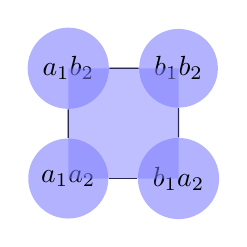
\begin{tikzpicture}
  [scale=.7,auto=left,every node/.style={circle,fill=blue!30}]
  \node (n1) at (1,3)  {$a_1b_2$};
  \node (n2) at (3,3)  {$b_1b_2$};
  \node (n3) at (1,1)  {$a_1a_2$};
  \node (n4) at (3,1)  {$b_1a_2$};

\foreach \from/\to in
{n1/n2, n3/n4, n1/n3, n2/n4}
    \draw (\from) -> (\to);
    \path[fill=blue!50,opacity=.5] (n1.center) to (n2.center) to (n4.center) to (n3.center) to (n1.center);
\end{tikzpicture}
\hspace{.5in}
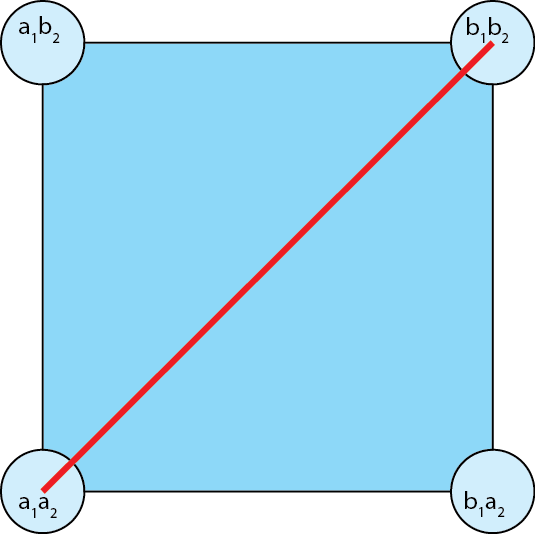
\includegraphics[scale=.3]{Export.png}
\end{figure}

Repeating this process for every other $2$-cell obtained by taking the product of a $1$-cell with itself and putting the configuration space together, we obtain Figure~\ref{fig:config}. The dotted lines are used to represent where a pairwise diagonal element was removed.

\begin{figure}[h]
\centering
\caption{$C^2(\Y)$ [Arb00]}
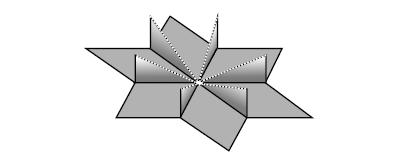
\includegraphics[scale=1]{Presentation/Config.jpg}
\label{fig:config}
\end{figure}

This is the configuration space of $C^2(\Y)$. While it is easier to visually intuit, this configuration space for two robots is already embedded in the three dimensional space $R^3$. For more robots, our ability to draw these configuration spaces quickly escapes us. Thus we will employ topological tools to simplify the dimension of the space into something more tractable.
\end{document}








